\section{Как заполнять документ}

Сейчас я расскажу, как максимально быстро собрать лекцию, чтобы никому ничего не сломать.
Предлагаю также ориентироваться на этот пример (папка \texttt{ch0}). Итак, порядок действий:
\begin{enumerate}
        \item Скачать себе этот архив.\\
        \textit{Он собирается командой \texttt{make} или \texttt{pdflatex doc}, если вы используете Windows.}
                \item Создать в корне вашу папку \texttt{chНОМЕРГЛАВЫ}. \\
        \textit{В примере папка \texttt{ch0}.}
        \item Заполнить в этой папке три документа: \texttt{doc.tex}, \texttt{bib.tex}, \texttt{set.tex}, положить туда все ваши картинки и все, что вам нужно.
        \item Проверить, что все собралось правильно.
        \item Отослать мне на почту \texttt{kireku@gmail.com} с темой ``ВКР'' или, если вы умеете, сделать \texttt{pull request}.
\end{enumerate}


\subsection{doc.tex}

Это файл с вашим текстом.
Туда вы пишите лекцию.

Я добавил уже ряд математических операторов.
Если вы хотите добавить свои смотри раздел про \texttt{set.tex}.

\begin{center}
\begin{tabular}{|c|c|}
\hline
        Код                         & Результат \\ \hline

        \texttt{\symbol{'134}sgn}   & $\sgn$    \\ \hline
        \texttt{\symbol{'134}const} & $\const$  \\ \hline
        \texttt{\symbol{'134}T}     & $\T$      \\ \hline
        % Множества
        \texttt{\symbol{'134}SetN}  & $\SetN$   \\ \hline
        \texttt{\symbol{'134}SetZ}  & $\SetZ$   \\ \hline
        \texttt{\symbol{'134}SetQ}  & $\SetQ$   \\ \hline
        \texttt{\symbol{'134}SetR}  & $\SetR$   \\ \hline
        \texttt{\symbol{'134}SetC}  & $\SetC$   \\ \hline
        % Теорвер
        \texttt{\symbol{'134}Prb}   & $\Prb$    \\ \hline
        \texttt{\symbol{'134}Ind}   & $\Ind$    \\ \hline
        \texttt{\symbol{'134}Exp}   & $\Exp$    \\ \hline
        \texttt{\symbol{'134}Var}   & $\Var$    \\ \hline
        % Оптималка
        \texttt{\symbol{'134}SetX}  & $\SetX$   \\ \hline
        \texttt{\symbol{'134}SetP}  & $\SetP$   \\ \hline
\end{tabular}
\end{center}

Также встроены окружения. Они как в книжке Арама, то есть красивые, не используйте другие.
\begin{center}
\begin{tabular}{|c|c|}
\hline
        Код & Результат

\\ \hline        
        \begin{minipage}{3in}
                \begin{verbatim}

\begin{theorem}
        Это теорема.
\end{theorem}
                \end{verbatim}
        \end{minipage}
        & 
        \begin{minipage}{3in}
                \begin{theorem}
                        Это теорема.
                \end{theorem}
        \end{minipage}
\\ \hline
        \begin{minipage}{3in}
                \begin{verbatim}

\begin{definition}
        Это определение
        \textit{сходимости}.
\end{definition}
                \end{verbatim}
        \end{minipage}
        & 
        \begin{minipage}{3in}
                \begin{definition}
                        Это определение \textit{сходимости}.
                \end{definition}
        \end{minipage}
\\ \hline
        \begin{minipage}{3in}
                \begin{verbatim}

\begin{lemma}
        Это лемма.
\end{lemma}
                \end{verbatim}
        \end{minipage}
        & 
        \begin{minipage}{3in}
                \begin{lemma}
                        Это лемма.
                \end{lemma}
        \end{minipage}
\\ \hline
        \begin{minipage}{3in}
                \begin{verbatim}

\begin{assertion}
        Это утверждение.
\end{assertion}
                \end{verbatim}
        \end{minipage}
        & 
        \begin{minipage}{3in}
                \begin{assertion}
                        Это утверждение.
                \end{assertion}
        \end{minipage}
\\ \hline
        \begin{minipage}{3in}
                \begin{verbatim}

\begin{example}
        Это пример.
\end{example}
                \end{verbatim}
        \end{minipage}
        & 
        \begin{minipage}{3in}
                \begin{example}
                        Это пример.
                \end{example}
        \end{minipage}
\\ \hline
        \begin{minipage}{3in}
                \begin{verbatim}

\begin{proof}
        Это доказательство чего-либо.
\end{proof}
                \end{verbatim}
        \end{minipage}
        & 
        \begin{minipage}{3in}
                \begin{proof}
                        Это доказательство чего-либо.
                \end{proof}
        \end{minipage}
\\ \hline
\end{tabular}
\end{center}

Чтобы добавить картинку, положите ее в вашу папку и укажите полный путь:
\begin{center}
\begin{tabular}{|c|c|}
\hline
        Код & Результат

\\ \hline        
        \begin{minipage}{3in}
                \begin{verbatim}
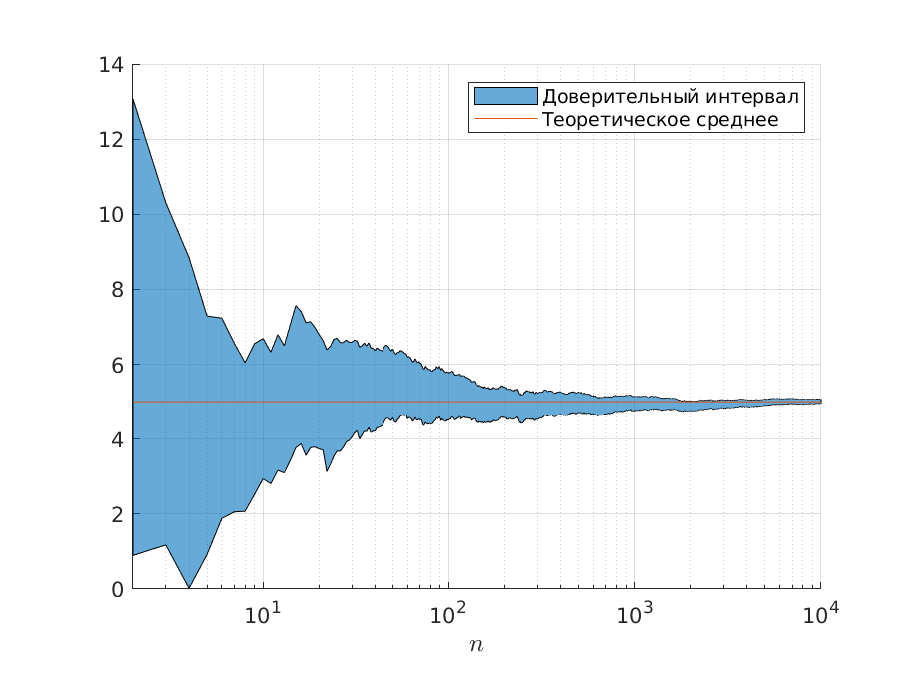
\includegraphics{ch0/example.eps}                
                \end{verbatim}
        \end{minipage}
        &
        \begin{minipage}{3in}
                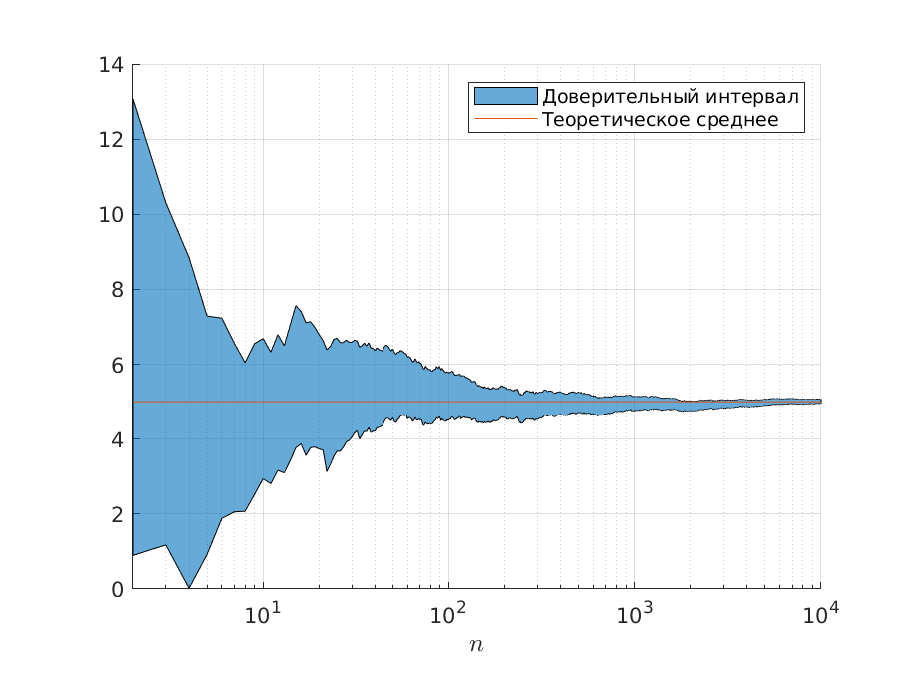
\includegraphics[width=3in]{ch0/example.eps}
        \end{minipage}
\\ \hline
\end{tabular}
\end{center}

Используя метки, обязательно ставьте префикс-название папки:
\begin{center}
\begin{tabular}{|c|c|}
\hline
        Код & Результат

\\ \hline        
        \begin{minipage}{3in}
                \begin{verbatim}

\begin{equation}
\label{ch0.square}
        x^2 = 0.
\end{equation}
                \end{verbatim}
        \end{minipage}
        &
        \begin{minipage}{3in}
                \begin{equation}\label{ch0.square}
                    x^2 = 0.
                \end{equation}
        \end{minipage}
\\ \hline
\end{tabular}
\end{center}


\subsection{bib.tex}

Если вам нужна библиография~--- сюда можно написать библиографию, она автоматом окажется внизу. Все ссылки, по-прежнему с префиксом.
\begin{center}
\begin{tabular}{|c|}
\hline
        Содержимое \texttt{ch0/bib.tex}

\\ \hline        
        \begin{minipage}{6in}
                \begin{verbatim}

\bibitem{ch0.voroncov}
        К.~В.~Воронцов. \textit{\LaTeX в примерах}.~--- М.: МЦНМО, 2005.
                \end{verbatim}
        \end{minipage}
\\ \hline
\end{tabular}
\end{center}


\subsection{set.tex}

Если вам жизненно не хватает какой-нибудь суперштуки, которую обычно объявляют в начале файла: новую команду, окружение или что-то в этом духе, то напишите сюда. Но все это пишите с каким-нибудь префиксом.

Например, я очень захотел писать прикольные дроби, типа \nicefrac{3}{4} и новый оператор $\zeroKir\limits_{x\in\SetX}$, тогда я должен туда написать:

\begin{center}
\begin{tabular}{|c|}
\hline
        Содержимое \texttt{ch0/bib.tex}

\\ \hline        
        \begin{minipage}{6in}
                \begin{verbatim}

\usepackage{nicefrac}
\DeclareMathOperator{\zeroKir}{Kirill}
                \end{verbatim}
        \end{minipage}
\\ \hline
\end{tabular}
\end{center}
Но вообще, если вы не уверены, что все не перестанет компилиться, то не стоит подключать пакеты.
Пакеты будут действовать на весь документ в целом.


\subsection{Заключение}

Вообще, было бы круто, чтобы все получилось примерно одинаково и красиво. В библиографии есть книжка хорошая по Латеху, если кому нужна.

\subsection{Список приславших} 

\begin{enumerate}
    \item Абрамова
    \item Авалиани
    \item Егоров
    \item Кожевец
\end{enumerate}